\documentclass[20pt,t]{beamer}
\usepackage[size=a1, orientation=portrait, scale=1.25]{beamerposter}
\beamertemplatenavigationsymbolsempty % hide navigation symbols (usually appears on the right corner)

%% useful packages-----------------------------------------------------------------------------------
\usepackage{url}
\usepackage{amsmath}
\usepackage{changepage} % setting the block margin width
\renewcommand{\raggedright}{\leftskip=0pt \rightskip=0pt}

\usepackage{cite}
\renewcommand{\citedash}{--}\usepackage{cite}
\renewcommand{\citedash}{--}

\usepackage{wrapfig}

%\usepackage{authblk}

%\usepackage{hyperref} % \url package 
%%\usepackage[colorlinks=true,linkcolor=black,anchorcolor=black,citecolor=black,filecolor=black,menucolor=black,runcolor=black,urlcolor=black]{hyperref} % use \url but remoce the colors but keep the hyperlinks
%\usepackage[colorlinks=true, allcolors=black]{
	
%\urlstyle{rm}
%%%%%%%%%%%%%%%%%%%%%%%%%%%%%%%%%%%%%%%%%%%%%%%%%%%%%%%%%%%%%%%%%%%%%%%%%%%%%%%%%%%%%%%%%%%%%%%%%%%%
%% necessary packages-------------------------------------------------------------------------------
\usetheme{Madrid} % using the theme

%%%%%%%%%%%%%%%%%%%%%%%%%%%%%%%%%%%%%%%%%%%%%%%%%%%%%%%%%%%%%%%%%%%%%%%%%%%%%%%%%%%%%%%%%%%%%%%%%%%%
%%%% Fonts------------------------------------------------------------------------------------------

% block design-------------------------------------------------------------------------------------
\setbeamerfont{block title}{series=\bfseries}
\setbeamerfont{block body}{family=\sffamily}

% block design-------------------------------------------------------------------------------------
\setbeamerfont{beamerboxesrounded title}{size=\Large,series=\bfseries}
\setbeamerfont{beamerboxesrounded body}{family=\rmfamily}

%%%%%%%%%%%%%%%%%%%%%%%%%%%%%%%%%%%%%%%%%%%%%%%%%%%%%%%%%%%%%%%%%%%%%%%%%%%%%%%%%%%%%%%%%%%%%%%%%%%%
%% changing the width of the items in itemize
%\let\olditemize\itemize
%\renewcommand{\itemize}{\olditemize\addtolength{\itemsep}{0.4\baselineskip}}
\setbeamertemplate{itemize item}[circle]
\setbeamercolor{itemize item}{bg=black,fg=black}

%%%%%%%%%%%%%%%%%%%%%%%%%%%%%%%%%%%%%%%%%%%%%%%%%%%%%%%%%%%%%%%%%%%%%%%%%%%%%%%%%%%%%%%%%%%%%%%%%%%%
%% blocks design and settings-----------------------------------------------------------------------
%\setbeamertemplate{blocks}[rounded][shadow=false] % enable shadow mode of blocks
% Do not use this if you are using the theme

%%%%%%%%%%%%%%%%%%%%%%%%%%%%%%%%%%%%%%%%%%%%%%%%%%%%%%%%%%%%%%%%%%%%%%%%%%%%%%%%%%%%%%%%%%%%%%%%%%%%
%% Set top and bottom spacing for blocks
\addtobeamertemplate{block begin}{\vspace{2mm}}{\vspace{2mm}\begin{adjustwidth}{2mm}{2mm}}
\addtobeamertemplate{block end}{\end{adjustwidth}}{\vspace{1mm}}

%% Set top and bottom spacing for the alert box
\addtobeamertemplate{block alerted begin}{\vspace{2mm}}{\vspace{2mm}\begin{adjustwidth}{2mm}{2mm}}
\addtobeamertemplate{block alerted end}{\end{adjustwidth}}{\vspace{1mm}}

%% set top and bottom spacing for example blocks
\addtobeamertemplate{block example begin}{\vspace{2mm}}{\vspace{2mm}\begin{adjustwidth}{2mm}{2mm}}
\addtobeamertemplate{block example end}{\end{adjustwidth}}{\vspace{1mm}}

%% set top and bottom spacing for roundedcolourbox
%\addtobeamertemplate{beamerboxesrounded begin}{}{\vspace{5mm}\begin{adjustwidth}{5mm}{5mm}}
%\addtobeamertemplate{beamerboxesrounded end}{\end{adjustwidth}}{\vspace{5mm}}

% setting the block title to centering
%\setbeamerfont{block title}{size={\bfseries\fontsize{48}{60}}}

%%%%%%%%%%%%%%%%%%%%%%%%%%%%%%%%%%%%%%%%%%%%%%%%%%%%%%%%%%%%%%%%%%%%%%%%%%%%%%%%%%%%%%%%%%%%%%%%%%%%
%% setting colors-----------------------------------------------------------------------------------

%% block body color
%\setbeamercolor{block body}{bg=cyan!10,fg=black}
%\setbeamercolor{block title}{bg=cyan!50,fg=black}
%
\setbeamercolor{footline}{fg=black,bg=}
\setbeamercolor{backgroud canvas}{bg=}
%\setbeamertemplate{background canvas}[vertical shading][top=blue!25,bottom=white,middle=white,midpoint=0.85]

%% header background color--------------------------------------------------------------------------
%\pgfdeclareimage[height=0.45cm]{headlineBGimage}{headlineBG.pdf}
%\setbeamercolor{HeadlineBGColor}{fg=black,bg=headlineBGimage}
\setbeamercolor{HeadlineBGColor}{fg=black,bg=}

%%%%%%%%%%%%%%%%%%
% captioning
\setbeamertemplate{caption}[default]
\setbeamercolor{caption name}{fg=black}


%%%%%%%%%%%%%%%%%%%%%%%%%%%%%%%%%%%%%%%%%%%%%%%%%%%%%%%%%%%%%%%%%%%%%%%%%%%%%%%%%%%%%%%%%%%%%%%%%%%%
%% setting Title environment------------------------------------------------------------------------
\setbeamertemplate{headline}{%
%
	\begin{beamercolorbox}[wd=0.98\paperwidth]{HeadlineBGColor} %\vskip5mm
		\begin{columns}[c]
		%% first column-----------------------------------------------------------------------------
			\begin{column}{0.15\linewidth}
				\vfill
				\centering
				
\includegraphics[width=\linewidth]{Figures/LiU_secondary_black.eps}
			\end{column}
		%% second column----------------------------------------------------------------------------
			\begin{column}{0.65\linewidth}
				\vskip5ex
				\begin{center}
					\setlength\lineskip{6pt}
					\usebeamercolor{title in headline}{\color{fg}\textbf{\Huge{\inserttitle}}\\[1ex]}
					\usebeamercolor{author in headline}{\color{fg}\Large{\insertauthor}\\[1ex]}
					% \usebeamercolor{institute in headline}{\color{fg}\large{\insertinstitute}\\[1ex]}
				\end{center} 
			\end{column}
		%% third column-----------------------------------------------------------------------------
			\begin{column}{0.15\linewidth}
				\centering
				
\includegraphics[width=0.8\linewidth]{Figures/qr_code.pdf}
				% \large Scan for Publication
			\end{column}
		\end{columns}
		\vskip1ex
	\end{beamercolorbox}
%% headline bottom line------------------------------------------------------------------------------
\color{black}\rule{\paperwidth}{4pt}
}

%%%%%%%%%%%%%%%%%%%%%%%%%%%%%%%%%%%%%%%%%%%%%%%%%%%%%%%%%%%%%%%%%%%%%%%%%%%%%%%%%%%%%%%%%%%%%%%%%%%%
%% Footline setup-----------------------------------------------------------------------------------
\setbeamertemplate{footline}{%
	\begin{beamercolorbox}[wd=\paperwidth]{upper separation line foot}
		\color{black}\rule{\paperwidth}{3pt}
	\end{beamercolorbox}
	\leavevmode%
	\begin{beamercolorbox}[ht=-1.75ex,leftskip=1em,rightskip=1em]{footline}%
		\begin{columns}[T]
		%% first column ------
		\begin{column}{\paperwidth}
			\centering
			\vspace{5mm}
			\footnotesize arvind.balachandran@liu.se
			\vspace{3mm}
		\end{column}
		\end{columns}
	\end{beamercolorbox}

}

%%%%%%%%%%%%%%%%%%%%%%%%%%%%%%%%%%%%%%%%%%%%%%%%%%%%%%%%%%%%%%%%%%%%%%%%%%%%%%%%%%%%%%%%%%%%%%%%%%%%
%% including the definitions file 

%%%%%%%%%%%%%%%%%%%%%%%%%%%%%%%%%%%%%%%%%%%%%%%%%%%%%%%%%%%%%%%%%%%%%%%%%%%%%%%%%%%%%%%%%%%%%%%%%%%%
%% Title goes here----------------------------------------------------------------------------------
\title{Battery Integrated Modular Multilevel Converters for Automotive Applications}
\author{Arvind Balachandran}
\institute{Linköping University, Linköping, Sweden.}

%%%%%%%%%%%%%%%%%%%%%%%%%%%%%%%%%%%%%%%%%%%%%%%%%%%%%%%%%%%%%%%%%%%%%%%%%%%%%%%%%%%%%%%%%%%%%%%%%%%%
%%%%%%%%%%%%%%%%%%%%%%%%%%%%%%%%%%%%%%%%%%%%%%%%%%%%%%%%%%%%%%%%%%%%%%%%%%%%%%%%%%%%%%%%%%%%%%%%%%%%
%
%
%-------------- main document starts here
%
%
%%%%%%%%%%%%%%%%%%%%%%%%%%%%%%%%%%%%%%%%%%%%%%%%%%%%%%%%%%%%%%%%%%%%%%%%%%%%%%%%%%%%%%%%%%%%%%%%%%%%
%%%%%%%%%%%%%%%%%%%%%%%%%%%%%%%%%%%%%%%%%%%%%%%%%%%%%%%%%%%%%%%%%%%%%%%%%%%%%%%%%%%%%%%%%%%%%%%%%%%%

\usepackage{layouts}

\begin{document} 
	\begin{frame}
		\begin{columns}[c]
			%% first column-------------------------------------------------------------------------
			\begin{column}{.49\textwidth}
%				\vskip2ex % creating spacing from line to first header 
				%%% 1st section ----------------------------------------------------
				\begin{block}{\vspace{2mm} \Large\bfseries Contributions \vspace{1mm}}
					\begin{description}
						\item[\textbf{Design optimization}] Loss minimization, dc-link capacitor size vs switching frequency.
						\item[\textbf{Experimental validation}] Harmonic allocations and loss distribution within a submodule.
						\item[\textbf{Compaitirve analysis}] BI-MMC topologies with 2-level inverter.
						\item[\textbf{DC charging}] Maximum DC charging power for BI-MMC topologies.
					\end{description}
				\end{block}
				\vskip1ex
				%%% 2nd section ----------------------------------------------------
				\begin{beamerboxesrounded}[lower=white,upper=white,shadow=false]{\Large\bfseries Topology overview}
					\begin{figure}[!h]
						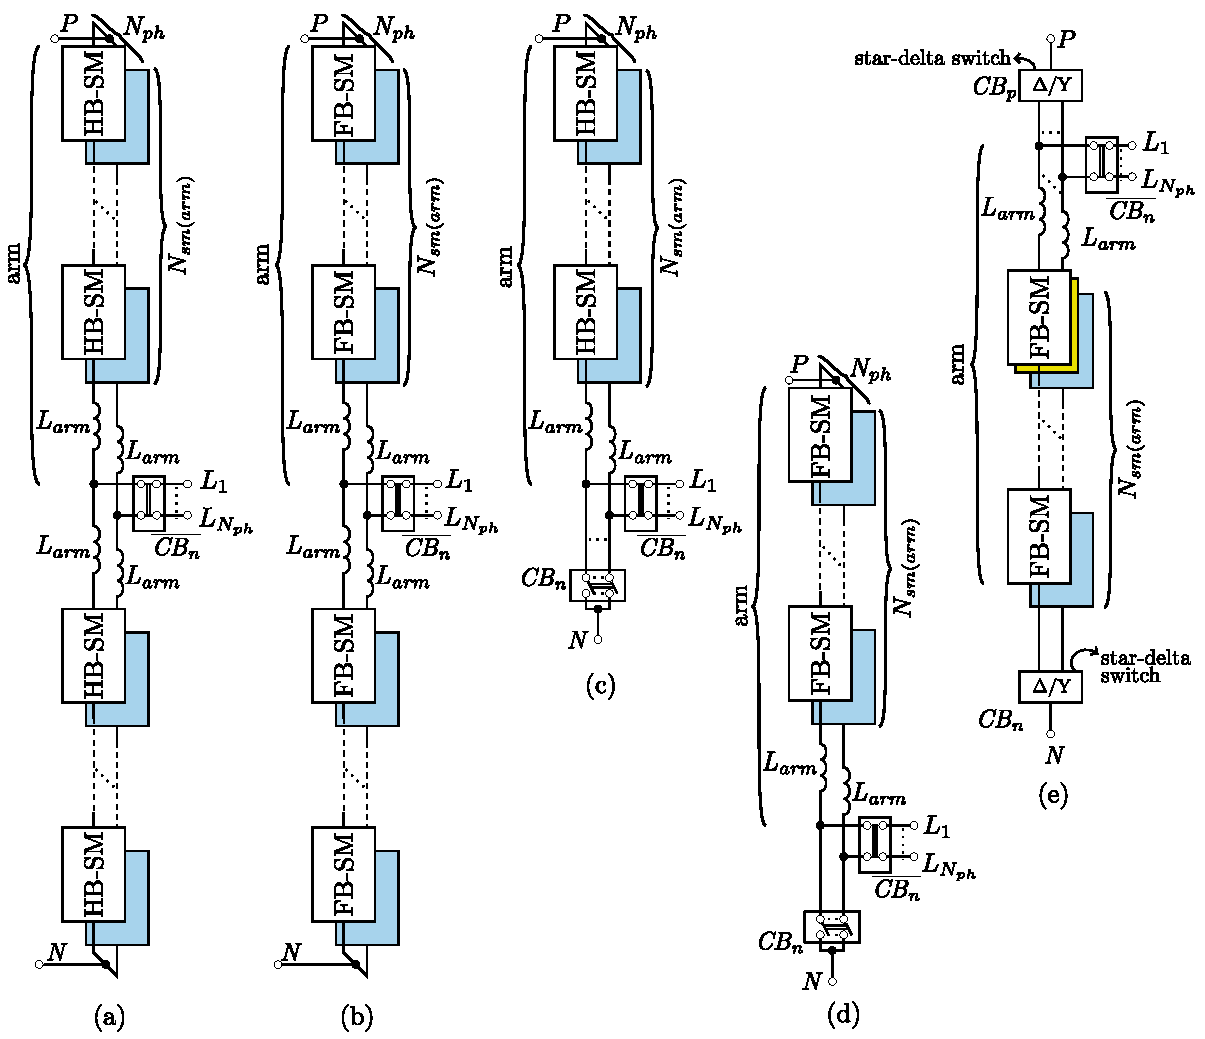
\includegraphics[width=\textwidth]{Figures/All_tops.pdf}
						\caption{Double-star (DS), single-star (SS) with half-bridge (HB) and full-bridge (FB), and single-delta with FB.}
					\end{figure}
					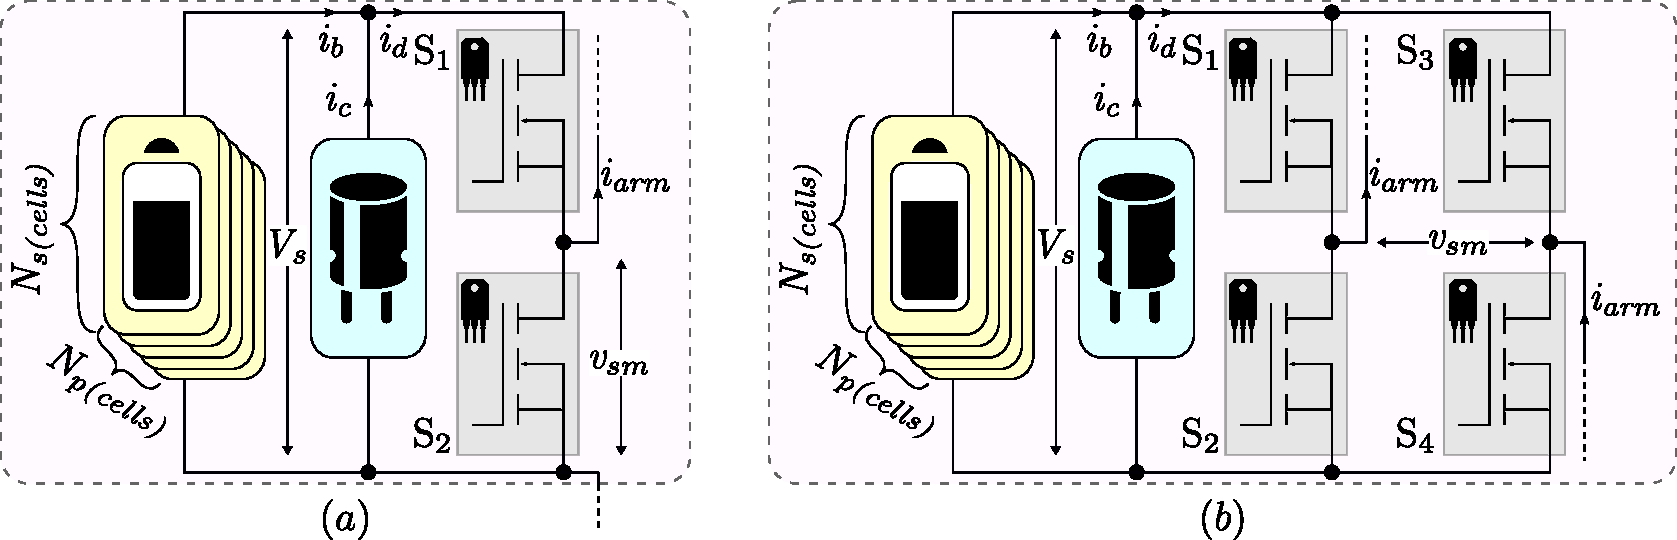
\includegraphics[width=\textwidth]{Figures/HB_FB_submodule.pdf}
					\begin{block}{}
						\[
							\text{(a) HB-SM} \quad \textit{V}_{\textit{sm(hb)}} = \textit{M}\,\frac{\textit{V}_{\textit{s}}}{2\,\sqrt2} \qquad \text{(b) FB-SM} \quad
							\textit{V}_{\textit{sm(fb)}} = \textit{M}\,\frac{\textit{V}_{\textit{s}}}{\sqrt2} 
						\]
					\end{block}
				\end{beamerboxesrounded}
				\vskip1ex
				%%% 3rd section ----------------------------------------------------
				\begin{beamerboxesrounded}[lower=white,upper=white,shadow=false]{\Large\bfseries Submodule Loss distribution}
					\begin{figure}[!h]
						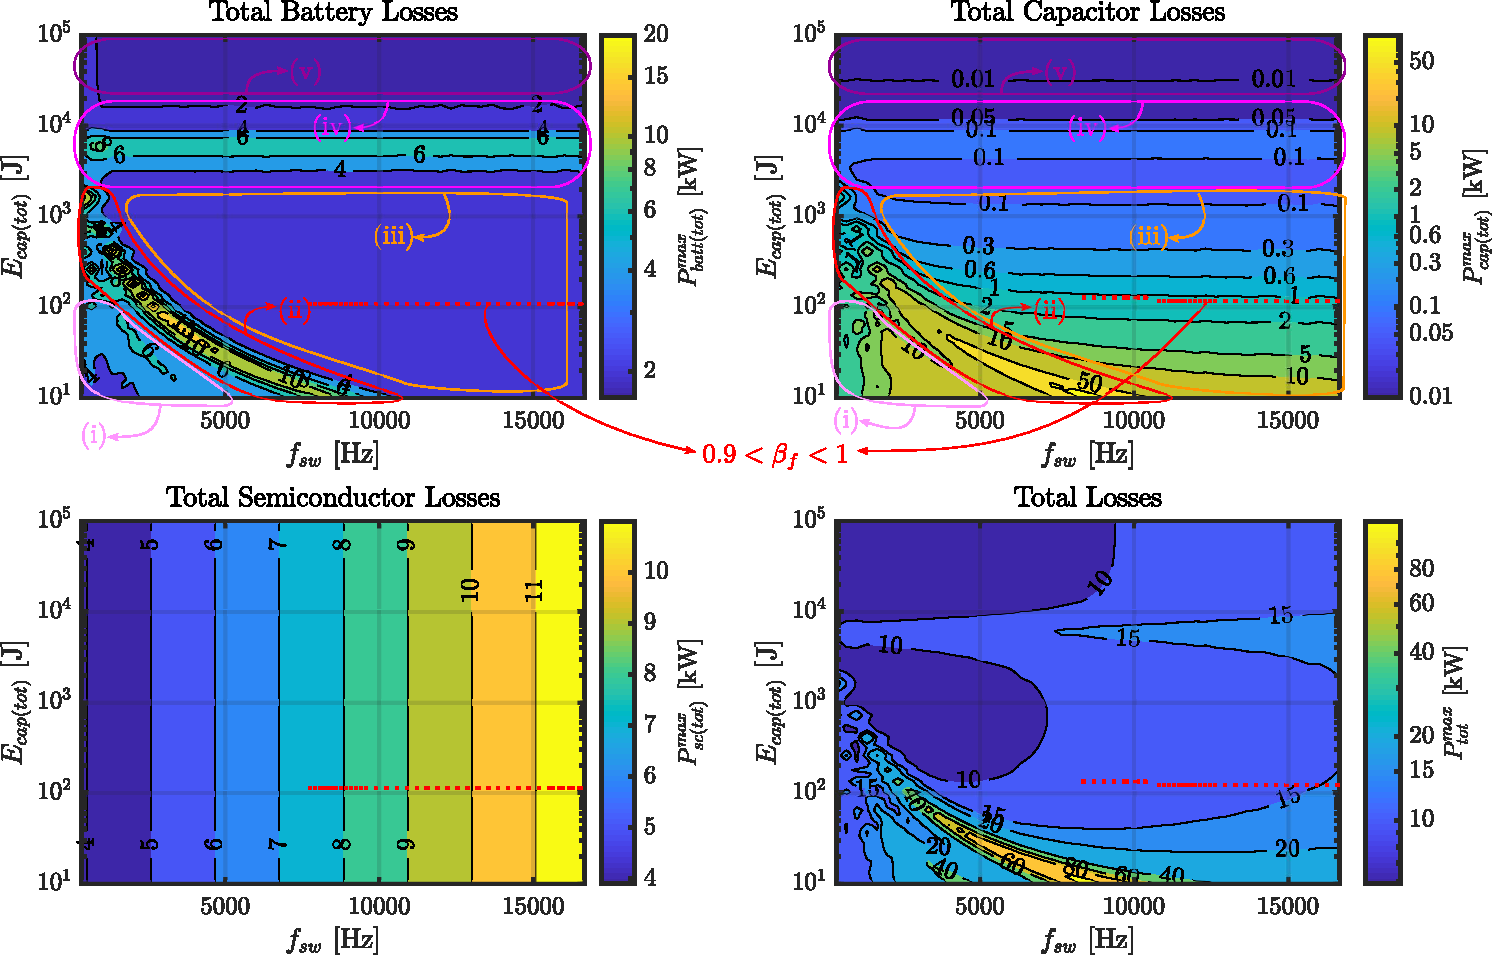
\includegraphics[width=\textwidth]{Figures/DC_cap_design.pdf}
						\caption{Losses for a 5-$\textit{N}_{\textit{s(cells)}}$, DSFB BI-MMC topology at a rated power of 400\,kW.}
					\end{figure}
					\begin{columns}[T]
						\begin{column}{0.1\textwidth}
							region(i):
							$f_{\textit{sw}} < f_{\textit{res}}$
						\end{column}
						\begin{column}{0.1\textwidth}
							region(ii):
							$f_{\textit{sw}} \approx f_{\textit{res}}$
						\end{column}
						\begin{column}{0.1\textwidth}
							region(iii):
							$f_{\textit{sw}} > f_{\textit{res}}$
						\end{column}
						\begin{column}{0.1\textwidth}
							region(iv):
							$f_{\textit{sw}} \approx 2\,f_{1}$
						\end{column}
						\begin{column}{0.1\textwidth}
							region(v):
							$f_{\textit{sw}} > 2\,f_{1}$
						\end{column}
					\end{columns}
					\begin{alertblock}{}
						\begin{columns}
							\begin{column}{0.4\textwidth}
								\[ f_{\textit{res}} = \frac{1}{2\pi\,\sqrt{\textit{L}_{\mathcal{B}}\textit{C}_{\textit{cap}}}} \]
							\end{column}
							\begin{column}{0.5\textwidth}
								\[P_{\textit{tot}}^{\textit{$\max{}$}} = P_{\textit{batt(tot)}}^{\textit{$\max{}$}} + P_{\textit{cap(tot)}}^{\textit{$\max{}$}} + P_{\textit{sc(tot)}}^{\textit{$\max{}$}} \]
							\end{column}
						\end{columns}
					\end{alertblock}
				\end{beamerboxesrounded}
			\end{column}
			%% second column------------------------------------------------------------------------	
			\begin{column}{.49\textwidth}
				\vspace{2mm}
				% \vskip2ex % creating spacing from line to first header 
				%%% 1st section ----------------------------------------------------
				\begin{beamerboxesrounded}[lower=white,upper=white,shadow=false]{\Large\bfseries Battery and capacitor currents in a submodule}
					\begin{alertblock}{}
						\begin{columns}[T]
							\begin{column}{0.33\textwidth}
								\centering
								$\displaystyle
								\begin{aligned}
									\textit{I}_{\textit{batt}}(f_{\textit{sw}}) &< \textit{I}_{\textit{cap}}(f_{\textit{sw}}) \\
									\textbf{$f_{\textit{sw}}$} &< \textbf{$f_{\textit{ref}}$}
								\end{aligned}$
							\end{column}
							\begin{column}{0.33\textwidth}
								\centering
								$\displaystyle
								\begin{aligned}
									\textit{I}_{\textit{batt}}(f_{\textit{sw}}) &\approx \textit{I}_{\textit{cap}}(f_{\textit{sw}}) \\
									\textbf{$f_{\textit{sw}}$} &\approx \textbf{$f_{\textit{ref}}$}
								\end{aligned}$
							\end{column}
							\begin{column}{0.33\textwidth}
								\centering
								$\displaystyle
								\begin{aligned}
									\textit{I}_{\textit{batt}}(f_{\textit{sw}}) &> \textit{I}_{\textit{cap}}(f_{\textit{sw}}) \\
									\textbf{$f_{\textit{sw}}$} &> \textbf{$f_{\textit{ref}}$}
								\end{aligned}$
							\end{column} 
						\end{columns}
					\end{alertblock}
					\vskip0.5ex
					\begin{figure}[htbp]
						\centering
						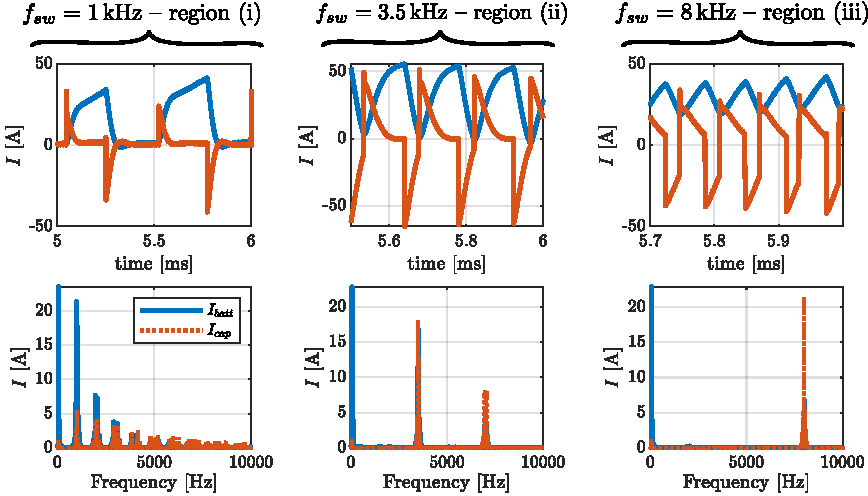
\includegraphics[width=\textwidth]{Figures/harm_alloc_td_fd_poster.pdf}
						\caption{Current measurements on a 1-$\textit{N}_{\textit{s(cells)}}$, 15\,V SSFB BI-MMC topology.}
					\end{figure}
				\end{beamerboxesrounded}
				\vskip1ex
				%%% 2nd section ----------------------------------------------------
				\begin{beamerboxesrounded}[lower=white,upper=white,shadow=false]{\Large\bfseries Power Losses}
					\vskip0.5ex 
					\begin{columns}[c]
						\begin{column}{0.75\textwidth}
							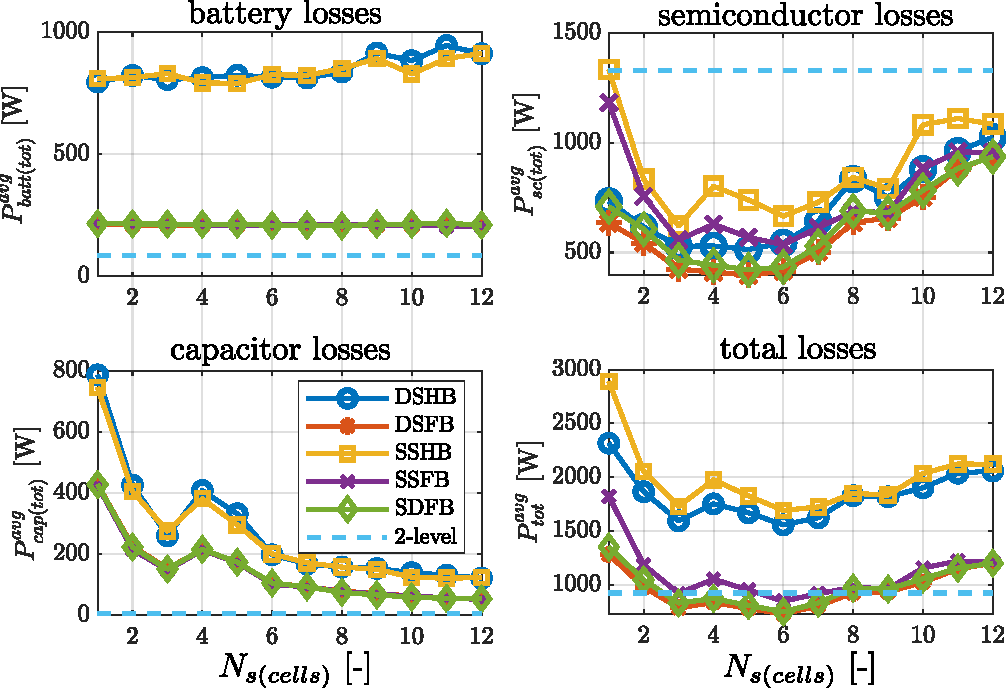
\includegraphics[width=\textwidth]{Figures/results_epe.pdf}	
						\end{column}
						\begin{column}{0.24\textwidth}
							Total losses at 100\,kW. 
							\begin{alertblock}{}
								BI-MMC topologies have higher $P_{\textit{batt(tot)}}^{\textit{avg}}$ and $P_{\textit{cap(tot)}}^{\textit{avg}}$. \\
							\end{alertblock}
							\begin{exampleblock}{}
								BI-MMC $P_{\textit{sc(tot)}}^{\textit{avg}}$ lower than 2-level inverter. \\
							\end{exampleblock}
						\end{column}
					\end{columns}
				\end{beamerboxesrounded}
				\vskip1ex
				%%% 3rd section ----------------------------------------------------
				\begin{beamerboxesrounded}[lower=white, upper=white, shadow=flase]{\Large\bfseries Performance Matrix \normalsize (efficiency vs total submodules)}
					\vskip0.5ex
					\begin{columns}[c]
						\begin{column}{0.62\textwidth}
							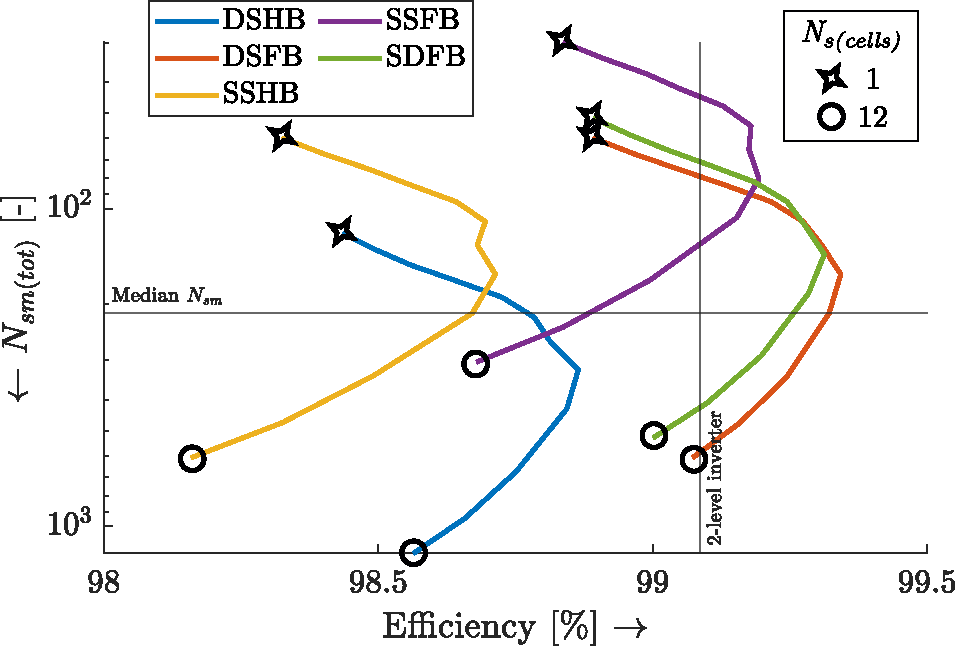
\includegraphics[width=\textwidth]{Figures/results_perfeval.pdf}
						\end{column}
						\begin{column}{0.37\textwidth}
							\begin{exampleblock}{}
								6 $\textit{N}_{\textit{s(cells)}}$ lowest losses,  given topology. \\

								FB topology lowest losses, given $\textit{N}_{\textit{s(cells)}}$. \\
							\end{exampleblock}
						\end{column}
					\end{columns}
				\end{beamerboxesrounded}
				\vskip1ex
				%%% 4th section ----------------------------------------------------
				\begin{beamerboxesrounded}[lower=white,upper=white,shadow=false]{\Large\bfseries Maximum DC charging power}
					\vskip0.5ex 
					\begin{figure}
						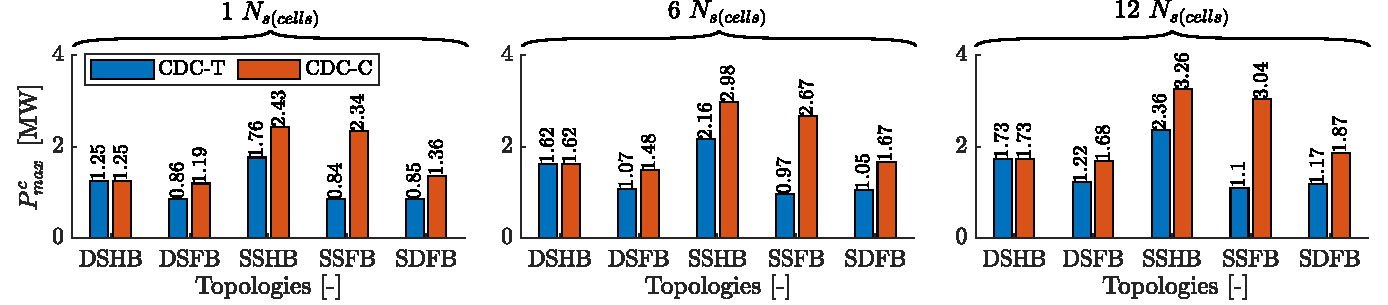
\includegraphics[width=\textwidth]{Figures/Results_Pdc_v4.pdf}
						\caption{The losses during charging at $\textit{P}_{\textit{max}}^{\textit{c}}$ is equal to traction losses at 400\,kW.}
					\end{figure}
					\centering
					$\textit{N}_{\textit{sm(tot)}}$ based on traction voltage (CDC-T) and based on charger voltage (CDC-C). \\
				\end{beamerboxesrounded}
				\vskip1ex
				%% final section ----------------------------------------------------
				\begin{block}{\vspace{2mm} \Large\bfseries Conclusions \vspace{1mm}}
					\textbf{Design optimization}:
					DC-link capacitor and switching frequency choice such that $\textit{f}_{\textit{sw}} \neq \textit{f}_{\textit{res}}$.\\
					
					\textbf{Comparative analysis}: BI-MMC topologies vs 2-level inverter:\par
					\hspace{50pt} Higher battery and capacitor losses, but Lower semiconductor losses.\par
					\hspace{50pt} Lower total losses for FB topologies with 5-6 $\textit{N}_{\textit{s(cells)}}$.\\

					\textbf{DC charging}: maximum DC charging power for BI-MMCs is between 800\,W to 3.26\,MW with the same losses as traction.
				\end{block}
%				\begin{beamerboxesrounded}[lower=white,upper=white,shadow=false]{\Large\bfseries Title}
%					
%					Normal text 
%					\begin{itemize}
%						\item  item 1
%						\item  item 2						
%					\end{itemize}
%					\vskip2ex
%				\end{beamerboxesrounded}
%				\begin{beamerboxesrounded}[lower=white,upper=white,shadow=false]{\Large\bfseries References}
%					\bibliographystyle{unsrt}
%					\bibliography{../Paper/references.bib}
%				\end{beamerboxesrounded}
			\end{column}
		\end{columns}
	\end{frame}
\end{document}